% Chapter 7: a new capstone for the audited Chapters 1--6.
% New exposition; not attributed to the source author of the earlier chapters.
% Build: pdflatex -halt-on-error mp_ch7.tex (twice).
\documentclass[11pt]{beamer}
\usepackage[utf8]{inputenc}
\usepackage[T1]{fontenc}
\usepackage{lmodern}
\usepackage{amsmath,amssymb,booktabs,array}
\usepackage{tikz,pgfplots}
\pgfplotsset{compat=1.18}
\usetheme{Madrid}
\usepackage{Kyushu}
\author[]{Compiled by Jake W. Liu}
\title[Calculus of Variations]{Chapter 7: Calculus of Variations}
\subtitle{Mathematical Physics}
\date{\today}
\setbeamertemplate{navigation symbols}{}
\setbeamertemplate{frametitle continuation}[from second]
\newcommand{\dd}{\,\mathrm{d}}
\newcommand{\D}{\mathcal D}
\newcommand{\Q}{\mathcal Q}
\newcommand{\N}{\mathcal N}
\newcommand{\R}{\mathcal R}
\newcommand{\Ai}{\operatorname{Ai}}
\newcommand{\Bi}{\operatorname{Bi}}
\begin{document}
\newcounter{sfchapter}
\setcounter{sfchapter}{7}
\renewcommand{\thesection}{\arabic{sfchapter}.\arabic{section}}
\numberwithin{equation}{section}

\begin{frame}[c]\titlepage\end{frame}

\begin{frame}{Outline}
\tableofcontents
\end{frame}

\begin{frame}{One question connects the course}
\small
Earlier chapters started with an equation and found its solutions. Here we ask:
\begin{center}
\textbf{Why does that equation arise, and what does its solution optimize?}
\end{center}
The common route is
\[
 \text{energy of a function}\ \longrightarrow\ \text{small change of the function}
 \ \longrightarrow\ \text{differential equation}.
\]
\begin{itemize}
\item With fixed boundary values: Laplace's equation and analytic functions.
\item With fixed size: Sturm--Liouville eigenfunctions, including Bessel and polynomial families.
\item With a trial shape: an approximation whose integrals use beta and gamma functions.
\end{itemize}
Physically, a sagging string and a soap film settle into the shape of lowest energy, and a
vibrating drum's modes balance stiffness against mass; the calculus of variations turns such
principles into equations.
\end{frame}

% ======================================================================
\section{From a functional to an equation}
% ======================================================================

\begin{frame}{A functional assigns a number to a whole curve}
\small
An ordinary function takes a number as input. A \emph{functional} takes a function:
\[
 u(x)\quad\longmapsto\quad J[u]=\frac12\int_0^1 u'(x)^2\dd x.
\]
This energy penalizes rapid change. Suppose $u(0)=0$ and $u(1)=1$ are fixed.
To change the curve without moving its ends, write
\begin{equation}
 u_\varepsilon(x)=u(x)+\varepsilon\eta(x),\qquad \eta(0)=\eta(1)=0.
 \label{eq:variation}
\end{equation}
Here $\eta$ chooses the \emph{shape} of the change; the real number $\varepsilon$
chooses its size and sign.
\begin{center}
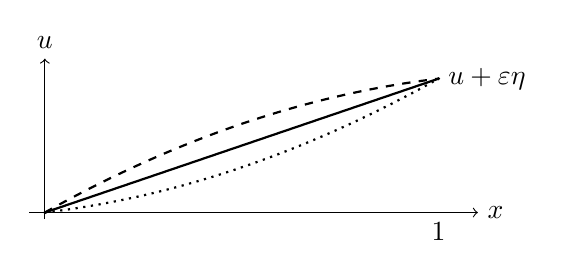
\begin{tikzpicture}[x=5cm,y=1.7cm]
\draw[->] (-.04,0)--(1.10,0) node[right] {$x$};
\draw[->] (0,-.05)--(0,1.15) node[above] {$u$};
\draw[thick] (0,0)--(1,1);
\draw[dashed,thick,domain=0:1,samples=60] plot (\x,{\x+0.65*\x*(1-\x)});
\draw[dotted,thick,domain=0:1,samples=60] plot (\x,{\x-0.65*\x*(1-\x)});
\fill (0,0) circle[radius=.6pt];\fill (1,1) circle[radius=.6pt];
\node[right] at (1,1) {$u+\varepsilon\eta$};
\node[below] at (1,0) {$1$};
\end{tikzpicture}
\end{center}
\end{frame}

\begin{frame}[allowframebreaks=1.00]{The first variation is an ordinary derivative}
\small
\textbf{The idea.} Fix \(u\) and the shape \(\eta\), and look at the ordinary function of one number,
\(\varepsilon\mapsto J[u+\varepsilon\eta]\). If \(u\) is a minimum, this function has its minimum at \(\varepsilon=0\), so its
derivative there must be zero, as in first-year calculus.

\textbf{Compute it for our energy.} Expand the square,
\((u'+\varepsilon\eta')^2=u'^2+2\varepsilon\,u'\eta'+\varepsilon^2\eta'^2\), and integrate:
\begin{align*}
 J[u+\varepsilon\eta]
 &=\frac12\int_0^1(u'+\varepsilon\eta')^2\dd x\\
 &=J[u]+\varepsilon\int_0^1u'\eta'\dd x
       +\frac{\varepsilon^2}{2}\int_0^1\eta'^2\dd x.
\end{align*}
This is a quadratic polynomial in \(\varepsilon\). Its derivative at \(\varepsilon=0\) is the coefficient of
\(\varepsilon\), called the \emph{first variation}:
\begin{equation}
 \delta J[u;\eta]
 :=\left.\frac{\mathrm d}{\mathrm d\varepsilon}J[u+\varepsilon\eta]\right|_{\varepsilon=0}
 =\int_0^1u'\eta'\dd x.\label{eq:first-variation}
\end{equation}
\par\framebreak\par
\textbf{Why it must vanish at a minimum.} For small \(\varepsilon\),
\(J[u+\varepsilon\eta]\approx J[u]+\varepsilon\,\delta J\). If \(\delta J\ne0\), choose a small \(\varepsilon\) with the opposite sign
to \(\delta J\): then \(\varepsilon\,\delta J<0\) and \(J\) goes down, so \(u\) was not a minimum. Hence, at a minimum,
\[
 \delta J[u;\eta]=0\qquad\text{for every allowed }\eta .
\]
A function \(u\) with this property is called \emph{stationary} (it could also be a maximum or a saddle;
we check which later).
\end{frame}

\begin{frame}[allowframebreaks=1.00]{One integration by parts gives the equation}
\small
\textbf{Step 1: move the derivative off \(\eta\).} Integrate \eqref{eq:first-variation} by parts
(\(\int fg'=[fg]-\int f'g\) with \(f=u'\), \(g=\eta\)):
\[
 \delta J=[u'\eta]_0^1-\int_0^1u''\eta\dd x
          =-\int_0^1u''\eta\dd x,
\]
since \(\eta(0)=\eta(1)=0\).

\textbf{Step 2: conclude \(u''=0\).} This integral must be zero for every \(\eta\). That forces \(u''=0\)
everywhere. \emph{Why:} if \(u''(x_0)\ne0\), say \(u''(x_0)>0\), then \(u''>0\) on a small interval around \(x_0\).
Choose \(\eta\) to be a small bump, positive on that interval and zero elsewhere. Then \(\int u''\eta\,dx>0\), a
contradiction.

\textbf{Step 3: solve.} \(u''=0\) gives \(u(x)=A+Bx\). The end conditions \(u(0)=0\), \(u(1)=1\) give \(A=0\), \(B=1\):
\[
 u_*(x)=x .
\]
\par\framebreak\par
\textbf{Step 4: it really is the minimum.} Take any competitor \(u_*+\eta\) (with \(\eta(0)=\eta(1)=0\)) and use
the exact expansion of the previous slide with \(\varepsilon=1\):
\[
 J[u_*+\eta]=J[u_*]+\int_0^1u_*'\eta'\dd x+\frac12\int_0^1\eta'^2\dd x .
\]
Since \(u_*'=1\), the middle term is \(\int_0^1\eta'\dd x=\eta(1)-\eta(0)=0\). So
\begin{equation}
 J[u_*+\eta]-J[u_*]=\frac12\int_0^1\eta'^2\dd x\ge0.\label{eq:line-minimum}
\end{equation}
Equality would need \(\eta'=0\), so \(\eta\) constant, so \(\eta=0\) (its end values are \(0\)). So \(u_*\) is the unique
minimum: the straight line. (Stationarity alone would not prove this; for example \(-J\) is stationary at
the same \(u_*\), where it has a maximum.)
\end{frame}

\begin{frame}[allowframebreaks=1.00]{The general Euler--Lagrange calculation}
\small
\textbf{Goal.} The last slides handled one energy. Now take a general energy
\[
 J[u]=\int_a^b F\bigl(x,u(x),u'(x)\bigr)\dd x
\]
and find the differential equation that every stationary \(u\) must satisfy.

\textbf{Notation.} Think of \(F(x,s,v)\) as a function of three independent variables: position \(x\),
value \(s\), slope \(v\). Write \(F_s=\partial F/\partial s\) and \(F_v=\partial F/\partial v\), evaluated at
\((x,u(x),u'(x))\).

\textbf{Step 1: differentiate in \(\varepsilon\).} Replace \(u\) by \(u+\varepsilon\eta\): the value becomes \(u+\varepsilon\eta\) and the
slope \(u'+\varepsilon\eta'\). By the chain rule, \(\frac{d}{d\varepsilon}F(x,u+\varepsilon\eta,u'+\varepsilon\eta')\) at \(\varepsilon=0\) is
\(F_s\cdot\eta+F_v\cdot\eta'\). So
\[
 \delta J[u;\eta]=\int_a^b\bigl(F_s\eta+F_v\eta'\bigr)\dd x .
\]
\par\framebreak\par
\textbf{Step 2: integrate the \(\eta'\) term by parts}, \(\int F_v\eta'\,dx=[F_v\eta]-\int\frac{d}{dx}(F_v)\,\eta\,dx\):
\[
 \delta J[u;\eta]
 =[F_v\eta]_a^b+\int_a^b\Bigl(F_s-\frac{\mathrm d}{\mathrm dx}F_v\Bigr)\eta\dd x.
\]
\textbf{Step 3: conclude.} For variations with \(\eta(a)=\eta(b)=0\) the bracket is zero, and the bump argument
of the previous slide forces the bracket in the integral to vanish. This is the
\emph{Euler--Lagrange equation}:
\begin{equation}
 \frac{\mathrm d}{\mathrm dx}F_v=F_s.\label{eq:euler-lagrange}
\end{equation}
\textbf{Check 1: our first example.} \(F=\frac12v^2\): \(F_v=v=u'\), \(F_s=0\), so \((u')'=0\), that is, \(u''=0\). \checkmark

\textbf{Check 2: Newton's law.} Let \(x\) be time and \(F=\tfrac12Mv^2-V(s)\) (kinetic minus potential energy).
Then \(F_v=Mu'\) and \(F_s=-V'(u)\), so \eqref{eq:euler-lagrange} reads \((Mu')'=-V'(u)\), that is,
\(Mu''=\)force. This is the principle of least action.
\end{frame}

\begin{frame}{The endpoint term determines the boundary condition}
\small
After the Euler--Lagrange equation \eqref{eq:euler-lagrange} holds, only the bracket
$[F_v\eta]_a^b$ of the previous slide remains in the first variation:
\[
 \delta J=F_v(b)\eta(b)-F_v(a)\eta(a).
\]
\textbf{Fixed endpoint value:} $u(b)$ is prescribed, so $\eta(b)=0$.
There is no extra equation for $u'(b)$.

\medskip
\textbf{Free endpoint value:} the location $b$ is fixed, but $u(b)$ is not prescribed.
Then $\eta(b)$ is arbitrary, so stationarity requires $F_v(b)=0$.
This is a \emph{natural boundary condition}.

\medskip
For $F=\tfrac12p(x)u'^2$ it reads $p(b)u'(b)=0$, that is, $u'(b)=0$ when $p(b)>0$.

\medskip
\textbf{The equation and the boundary conditions come from the same calculation.}
\end{frame}

\begin{frame}[allowframebreaks=1.00]{A complete example with one free endpoint}
\small
\textbf{The problem.} Minimize
\[
 J[u]=\int_0^1\left(\frac12u'^2-u\right)\dd x,
 \qquad u(0)=0,\quad u(1)\ \text{free}.
\]
\textbf{Picture.} A taut string (tension \(1\)) under a load of \(1\) per unit length. Its right end is a ring
that slides freely on a vertical rod. \(\tfrac12u'^2\) is the stretching energy; \(-u\) is the potential
energy of the load.

\textbf{Step 1: equation and boundary condition.} Here \(F(x,s,v)=\tfrac12v^2-s\), so \(F_s=-1\) and \(F_v=v=u'\).
\begin{itemize}
  \item Euler--Lagrange \eqref{eq:euler-lagrange}: \((u')'=-1\), that is, \(u''=-1\).
  \item Natural condition at the free end: \(F_v(1)=0\), that is, \(u'(1)=0\).
\end{itemize}
\textbf{Step 2: solve.} Integrate \(u''=-1\): \(u'=-x+C\); \(u'(1)=0\) gives \(C=1\). Integrate again:
\(u=x-\tfrac12x^2+D\); \(u(0)=0\) gives \(D=0\). So
\[
 u(x)=x-\tfrac12x^2 .
\]
\textbf{Step 3: it is the minimum.} Take a competitor \(u+\eta\) with \(\eta(0)=0\) (\(\eta(1)\) is unrestricted).
Subtract the energies, expanding \((u'+\eta')^2\):
\[
 J[u+\eta]-J[u]=\int_0^1\Bigl[\tfrac12(u'+\eta')^2-(u+\eta)-\tfrac12u'^2+u\Bigr]\dd x ,
\]
which simplifies to
\[
 J[u+\eta]-J[u]=\int_0^1(u'\eta'-\eta)\dd x+\frac12\int_0^1\eta'^2\dd x .
\]
\par\framebreak\par
Integrate \(u'\eta'\) by parts:
\[
 \int_0^1(u'\eta'-\eta)\dd x=[u'\eta]_0^1-\int_0^1(u''+1)\eta\dd x .
\]
The bracket is \(u'(1)\eta(1)-u'(0)\eta(0)=0\) (since \(u'(1)=0\) and \(\eta(0)=0\)), and \(u''+1=0\). So
\[
 J[u+\eta]-J[u]=\frac12\int_0^1\eta'^2\dd x\ge0 ,
\]
with equality only for \(\eta=0\). So \(u\) is the unique minimum: the string sags in a parabola (\(u''=-1\))
and meets the frictionless rod horizontally (\(u'(1)=0\)).
\end{frame}

% ======================================================================
\section{Energy and complex analysis}
% ======================================================================

\begin{frame}[allowframebreaks=1.00]{The same energy in the plane}
\small
\textbf{The energy.} Let \(\Omega\) be a bounded connected region of the plane. For a real field \(u(x,y)\), the
\emph{Dirichlet energy} is
\begin{equation}
 \D[u]=\frac12\iint_\Omega(u_x^2+u_y^2)\dd A
       =\frac12\iint_\Omega|\nabla u|^2\dd A,\label{eq:dirichlet-energy}
\end{equation}
with \(\nabla u=(u_x,u_y)\) and \(\dd A=\mathrm dx\,\mathrm dy\). It is the two-dimensional version of
\(\frac12\int u'^2dx\).

\textbf{Physical meaning.} \(\D\) is the field energy of an electrostatic potential \(u\). It is also the extra
area of a soap film at small height \(u(x,y)\): the area element is \(\sqrt{1+|\nabla u|^2}\approx1+\tfrac12|\nabla u|^2\).

\textbf{The problem.} Prescribe the boundary values, \(u=g\) on the boundary \(\partial\Omega\), and minimize \(\D\).
Competitors are \(u+\varepsilon\eta\) with \(\eta=0\) on \(\partial\Omega\).
\par\framebreak\par
\textbf{The first variation.} As in one dimension, expand the squares:
\((u_x+\varepsilon\eta_x)^2=u_x^2+2\varepsilon u_x\eta_x+\varepsilon^2\eta_x^2\), and the same in \(y\). So
\[
 \D[u+\varepsilon\eta]=\D[u]+\varepsilon\iint_\Omega(u_x\eta_x+u_y\eta_y)\dd A+\frac{\varepsilon^2}2\iint_\Omega|\nabla\eta|^2\dd A,
\]
and the coefficient of \(\varepsilon\) is the first variation:
\[
 \delta\D[u;\eta]=\iint_\Omega(u_x\eta_x+u_y\eta_y)\dd A .
\]
\textbf{Next step:} as in one dimension, move the derivatives off \(\eta\) by integrating by parts, now in
both directions.
\end{frame}

\begin{frame}[allowframebreaks=1.00]{Planar integration by parts produces Laplace's equation}
\small
\textbf{Goal.} Turn \(\delta\D\) into (boundary term) \(-\) (integral of \(\eta\) times something), as one integration
by parts did in one dimension, and read off the equation.

\textbf{Step 1: product rule.} \(\partial_x(\eta u_x)=\eta_xu_x+\eta u_{xx}\) and \(\partial_y(\eta u_y)=\eta_yu_y+\eta u_{yy}\). Solve
for \(\eta_xu_x+\eta_yu_y\):
\[
 u_x\eta_x+u_y\eta_y
 =\underbrace{\partial_x(\eta u_x)+\partial_y(\eta u_y)}_{\text{a divergence}}-\eta\,(u_{xx}+u_{yy}).
\]
\textbf{Step 2: the divergence part becomes a boundary term.} This is the two-dimensional
\([fg]_a^b\). Use Green's theorem (Chapter~1), \(\oint(P\dd x+Q\dd y)=\iint(Q_x-P_y)\dd A\), with \(P=-\eta u_y\),
\(Q=\eta u_x\); then \(Q_x-P_y=\partial_x(\eta u_x)+\partial_y(\eta u_y)\), and
\[
 \iint_\Omega\big(\partial_x(\eta u_x)+\partial_y(\eta u_y)\big)\dd A
 =\oint_{\partial\Omega}\eta\,(u_x\dd y-u_y\dd x)
 =\int_{\partial\Omega}\eta\;\nabla u\cdot\mathbf n\dd s .
\]
(The step \((\mathrm dx,\mathrm dy)\) along the boundary has \(\Omega\) on its left; turned \(90^\circ\) clockwise it
points outward, so the outward normal times length is \(\mathbf n\dd s=(\mathrm dy,-\mathrm dx)\).)
\par\framebreak\par
\textbf{Step 3: put it together.} Writing \(\partial_nu=\nabla u\cdot\mathbf n\) (the outward normal derivative) and
\(\Delta u=u_{xx}+u_{yy}\) (the Laplacian),
\begin{equation}
 \delta\D=\int_{\partial\Omega}\eta\,\partial_nu\dd s
            -\iint_\Omega\eta\,\Delta u\dd A.\label{eq:planar-first}
\end{equation}
Compare with one dimension: \(\delta J=[u'\eta]-\int u''\eta\,dx\). The boundary term is the same idea, and \(u''\)
became \(\Delta u\).

\textbf{Step 4: conclude.} \(\eta=0\) on \(\partial\Omega\), so the boundary term is zero. For the area integral to vanish
for every \(\eta\), the bump argument of Section~7.1 gives
\begin{equation}
 \Delta u=0\quad\text{in }\Omega.\label{eq:laplace}
\end{equation}
So the field of least energy is \emph{harmonic}: it solves Laplace's equation, met in Chapter~6.
\end{frame}

\begin{frame}{Why the harmonic solution is a minimum}
\small
Suppose a smooth harmonic function $u_*$ with the prescribed boundary values has
been found. Any competitor is $u_*+\eta$, where $\eta=0$ on the boundary.
Expanding the squares in \eqref{eq:dirichlet-energy} exactly gives
\begin{align*}
 \D[u_*+\eta]-\D[u_*]
 &=\iint_\Omega\nabla u_*\cdot\nabla\eta\dd A
     +\frac12\iint_\Omega|\nabla\eta|^2\dd A\\
 &=\frac12\iint_\Omega|\nabla\eta|^2\dd A\ge0.
\end{align*}
The cross term is $\delta\D[u_*;\eta]$; it vanishes by \eqref{eq:planar-first},
since $\eta=0$ on $\partial\Omega$ and $\Delta u_*=0$.
Equality means $\nabla\eta=0$. On a connected region, $\eta$ is then constant;
its zero boundary values force that constant to be zero.

\medskip
\textbf{Therefore the harmonic solution is the unique energy minimizer.}
This is why a soap film or a steady temperature settles in the harmonic shape.
\end{frame}

\begin{frame}{Analytic functions construct the minimizers}
\small
Return to Chapter 1. If $F(z)=u(x,y)+iv(x,y)$ is analytic, the Cauchy--Riemann
equations are
\[
 u_x=v_y,\qquad u_y=-v_x.
\]
Differentiate the first in $x$ and the second in $y$:
\[
 u_{xx}=v_{yx},\qquad u_{yy}=-v_{xy},\qquad
 \Delta u=v_{yx}-v_{xy}=0.
\]
The mixed derivatives agree because an analytic function is infinitely differentiable (Chapter 1).
Hence $\operatorname{Re}F$ is harmonic, so by the previous slide it minimizes Dirichlet energy for its own boundary data.

\medskip
For example, $F(z)=z^n$ gives
\[
 u(r,\theta)=r^n\cos(n\theta),\qquad n=0,1,2,\ldots,
\]
using $z=re^{i\theta}$; likewise $F=-iz^n$ gives $r^n\sin(n\theta)$ for $n\ge1$.
Together these are precisely the regular disk harmonics from Chapter 6.
The same solution now has both an \emph{analytic} and a \emph{variational} description.
\end{frame}

\begin{frame}{From boundary Fourier data to an analytic polynomial}
\small
\textbf{Goal.} Find the harmonic function in the disk with given boundary values $g(\theta)$.

On the unit circle, prescribe a finite trigonometric sum with real coefficients:
\[
 g(\theta)=a_0+\sum_{n=1}^M\bigl(a_n\cos n\theta+b_n\sin n\theta\bigr).
\]
Choose $F(z)=a_0+\sum_{n=1}^M(a_n-ib_n)z^n$.
Indeed, $\operatorname{Re}[(a_n-ib_n)e^{in\theta}]
=a_n\cos n\theta+b_n\sin n\theta$.
Therefore
\begin{equation}
 u_*(r,\theta)=a_0+\sum_{n=1}^Mr^n(a_n\cos n\theta+b_n\sin n\theta)
 \label{eq:disk-harmonic}
\end{equation}
fits the boundary and is the unique energy minimizer.
For a general \(g\) the sums run to \(n=\infty\). The Fourier coefficients come from orthogonality:
\(a_n=\frac1\pi\int_0^{2\pi}g\cos n\theta\,d\theta\), \(b_n=\frac1\pi\int_0^{2\pi}g\sin n\theta\,d\theta\), and \(a_0\) is the mean of \(g\). Combining
them with \(\cos n\theta-i\sin n\theta=e^{-in\theta}\) gives the Taylor coefficients of \(F\):
\[
 a_n-ib_n=\frac1\pi\int_0^{2\pi}g(\theta)e^{-in\theta}\dd\theta,
 \qquad n\ge1.
\]
\end{frame}

\begin{frame}[allowframebreaks=1.00]{A worked disk boundary-value problem}
\small
Let $u(1,\theta)=2+3\cos\theta-\sin2\theta$, so $a_0=2$, $a_1=3$, $b_2=-1$, the other
coefficients vanish, and $a_2-ib_2=i$. The recipe of the preceding slide gives
\[
 F(z)=2+3z+iz^2,\qquad
 u_*=\operatorname{Re}F=2+3x-2xy,
\]
since $iz^2=i(x^2-y^2)-2xy$. This is harmonic because $u_{*,xx}=u_{*,yy}=0$.
On $x=\cos\theta$, $y=\sin\theta$ we have $2xy=\sin2\theta$, so it has the required boundary values.
\par\framebreak
By \eqref{eq:dirichlet-energy} with $u_{*,x}=3-2y$ and $u_{*,y}=-2x$, its energy is
\begin{align*}
 2\D[u_*]
 &=\iint_{x^2+y^2<1}\bigl((3-2y)^2+4x^2\bigr)\dd A\\
 &=\iint_{x^2+y^2<1}\bigl(9-12y+4(x^2+y^2)\bigr)\dd A\\
 &=9\pi+4\iint_{x^2+y^2<1}(x^2+y^2)\dd A\\
 &=9\pi+4\int_0^{2\pi}\int_0^1r^3\dd r\dd\theta=9\pi+4\cdot2\pi\cdot\tfrac14=11\pi.
\end{align*}
The disk has area $\pi$, the term $-12y$ integrates to zero by reflection symmetry,
and the last line uses $x^2+y^2=r^2$, $\dd A=r\dd r\dd\theta$.
Thus $\D[u_*]=11\pi/2$, and every different smooth field with the same
boundary values has larger energy.
\end{frame}

\begin{frame}{An annulus brings back the logarithm}
\small
Let $a<r<b$, with $0<a<b$, and prescribe $u(a)=0$, $u(b)=1$ on the two circles.
Try a radial field \(u(r)\). Since \(r=\sqrt{x^2+y^2}\), \(\partial r/\partial x=x/r\) and \(\partial r/\partial y=y/r\). By the
chain rule \(u_x=u'(r)\,x/r\) and \(u_y=u'(r)\,y/r\), so \(|\nabla u|^2=u'^2(x^2+y^2)/r^2=u'(r)^2\). With
\(\dd A=r\dd r\dd\theta\) and the \(\theta\)-integral giving \(2\pi\),
\[
 \D[u]=\frac12\int_0^{2\pi}\!\!\int_a^b u'(r)^2\,r\dd r\dd\theta
 =\pi\int_a^b r\,u'(r)^2\dd r.
\]
The Euler--Lagrange equation \eqref{eq:euler-lagrange} for $F=\pi r u'^2$
($F_v=2\pi ru'$, $F_s=0$) is
\[
 (2\pi r u')'=0\quad\Longrightarrow\quad
 ru'=C,\quad u=C\log r+D.
\]
The two boundary values give $C\log a+D=0$ and $C\log b+D=1$, so
$C=1/\log(b/a)$ and $D=-C\log a$:
\begin{equation}
 u_*(r)=\frac{\log(r/a)}{\log(b/a)}.\label{eq:annulus}
\end{equation}
Since $ru_*'=1/\log(b/a)$ is constant, $\Delta u_*=(ru_*')'/r=0$ (Chapter 6 polar Laplacian,
no $\theta$). So $u_*$ is harmonic and beats \emph{all} smooth competitors, not merely radial ones.
\end{frame}

\begin{frame}{The field is global; its analytic potential need not be}
\small
The annular solution is single-valued because $r=|z|$ is single-valued.
Locally it is the real part of
\[
 \frac{\log z-\log a}{\log(b/a)}.
\]
Since $\log z=\log r+i\theta$, its local imaginary part (harmonic conjugate) is $\theta/\log(b/a)$. One turn around the hole
adds $2\pi/\log(b/a)$ to that conjugate.
Thus there is \textbf{no single-valued analytic potential on the whole annulus}
with this real part. This is the branch issue from Chapter 1, not a failure of harmonicity.

\medskip
The energy is nevertheless unambiguous. Insert $u_*'=1/(r\log(b/a))$ from
\eqref{eq:annulus} into the radial energy of the previous slide:
\begin{align*}
 \D[u_*]
 &=\pi\int_a^b r\,u_*'(r)^2\dd r
 =\frac{\pi}{\log^2(b/a)}\int_a^b\frac{\dd r}{r}
 =\frac{\pi}{\log(b/a)}.
\end{align*}
Physically, with $u$ the potential between two coaxial conductors at voltages $0$ and $1$,
$\D=\tfrac12CV^2$ with $V=1$ gives $C=2\pi/\log(b/a)$: the capacitance per unit length of a
coaxial cable (units with permittivity $1$).
\end{frame}



% ======================================================================
\section{Normalization and Sturm--Liouville modes}
% ======================================================================

\begin{frame}{To find a nonzero mode, remove the amplitude freedom}
\small
With homogeneous (zero) boundary data, minimizing a nonnegative quadratic energy alone
usually gives $u=0$. To select a \emph{shape}, compare energy with squared size.
On a finite interval define
\begin{equation}
 \Q[u]=\int_a^b\bigl(pu'^2+Vu^2\bigr)\dd x,\quad
 \N[u]=\int_a^bwu^2\dd x,\quad
 \R[u]=\frac{\Q[u]}{\N[u]}.\label{eq:rayleigh}
\end{equation}
For now take smooth real coefficients, $p,w>0$, a nonzero real $u$, and
$u(a)=u(b)=0$. The potential $V$ need not be positive.

\medskip
For any real $c\ne0$, both numerator and denominator acquire the factor $c^2$:
$\R[cu]=\R[u]$. Equivalently, minimize $\Q$ among shapes with $\N=1$;
rescaling $u$ by $1/\sqrt{\N[u]}$ enforces this normalization.

\medskip
$\R$ is the \emph{Rayleigh quotient}. Physically, for a string of tension $p$ and
density $w$ vibrating as $u(x)\cos\omega t$, $\Q$ measures stiffness (potential energy)
and $\N$ measures mass (inertia); like $k/m$ for a spring, $\R=\omega^2$ at a mode:
$wU_{tt}=(pU_x)_x$ with $U=u\cos\omega t$ gives $-(pu')'=\omega^2wu$, the $V=0$ case of
\eqref{eq:sl-variational} below.
We derive its equation directly by the quotient rule.
\end{frame}

\begin{frame}[allowframebreaks=1.00]{Vary the quotient, not the normalization separately}
\small
\textbf{Goal.} Find the equation satisfied by a function \(u\) at which the Rayleigh quotient
\(\R=\Q/\N\) is stationary.

\textbf{Step 1: vary numerator and denominator.} Replace \(u\) by \(u+\varepsilon\eta\) and expand the squares, exactly as
before. For example \(p(u'+\varepsilon\eta')^2=pu'^2+2\varepsilon\,pu'\eta'+\varepsilon^2p\eta'^2\). The coefficients of \(\varepsilon\) are
\[
 \delta\Q=2\int_a^b(pu'\eta'+Vu\eta)\dd x,
 \qquad \delta\N=2\int_a^bwu\eta\dd x.
\]
\textbf{Step 2: vary the quotient.} By the quotient rule, \(\delta(\Q/\N)=(\N\,\delta\Q-\Q\,\delta\N)/\N^2\). Call the
value of the quotient at \(u\) \(\lambda=\R[u]\) (a number), so \(\Q=\lambda\N\):
\[
 \delta\R=\frac{\N\delta\Q-\lambda\N\delta\N}{\N^2}=\frac{\delta\Q-\lambda\,\delta\N}{\N}
 =\frac{2}{\N}\int_a^b\bigl(pu'\eta'+Vu\eta-\lambda wu\eta\bigr)\dd x .
\]
\par\framebreak\par
\textbf{Step 3: integrate by parts.} \(\int pu'\eta'\,dx=[pu'\eta]-\int(pu')'\eta\,dx\), so
\[
 \delta\R=\frac{2}{\N}\left\{[pu'\eta]_a^b+
     \int_a^b\bigl(-(pu')'+Vu-\lambda wu\bigr)\eta\dd x\right\}.
\]
\textbf{Why vary the quotient?} Because \(\R[cu]=\R[u]\), the quotient does not care about the size of \(u\),
so \(\eta\) can be any function (no constraint is needed to keep \(\N=1\)). Equivalently, the numerator above
is the first variation of \(\Q-\lambda\N\) with \(\lambda\) held fixed: \(\lambda\) plays the role of a Lagrange
multiplier.
\end{frame}

\begin{frame}[allowframebreaks=1.00]{The equation is the one from Chapter 4}
\small
\textbf{The equation.} For variations with \(\eta(a)=\eta(b)=0\) the boundary term vanishes, and the bump argument
makes the integrand zero:
\begin{equation}
 -(pu')'+Vu=\lambda wu.\label{eq:sl-variational}
\end{equation}
This is the Sturm--Liouville equation. Chapter~4 wrote it as \((pu')'+qu=-\lambda wu\); the two agree with
\[
 V=-q .
\]
\textbf{At a mode, the quotient is the eigenvalue.} Multiply \eqref{eq:sl-variational} by \(u\), integrate over \([a,b]\),
and integrate the first term by parts (\(-\int(pu')'u\,dx=-[pu'u]+\int pu'^2dx\)):
\[
 -[pu'u]_a^b+\int_a^b(pu'^2+Vu^2)\dd x
 =\lambda\int_a^bwu^2\dd x.
\]
With \(u(a)=u(b)=0\) the bracket is zero, and the two integrals are \(\Q[u]\) and \(\N[u]\) from
\eqref{eq:rayleigh}. So \(\Q[u]=\lambda\N[u]\), that is, \(\lambda=\R[u]\). Other boundary conditions work the same
way, as long as they make the boundary term vanish.
\end{frame}

\begin{frame}[allowframebreaks=1.00]{Every trial shape gives an upper bound on $\lambda_1$}
\small
\textbf{Goal.} Show that for \emph{any} trial function \(u\) (with the boundary conditions),
\(\R[u]\ge\lambda_1\), the lowest eigenvalue. So every guess gives an upper bound.

\textbf{Setup.} Let \(\phi_1,\phi_2,\dots\) be the eigenfunctions (Chapter~4), real, with
\(\lambda_1\le\lambda_2\le\cdots\), normalized so that \(\int w\phi_i\phi_j\dd x=\delta_{ij}\).

\textbf{Step 1: the mode-energy identity.} Integrate by parts (the boundary term vanishes since
\(\phi_j(a)=\phi_j(b)=0\)), then use the equation \eqref{eq:sl-variational} for \(\phi_i\):
\begin{equation}
 \int_a^b(p\phi_i'\phi_j'+V\phi_i\phi_j)\dd x
 =\int_a^b\bigl(-(p\phi_i')'+V\phi_i\bigr)\phi_j\dd x
 =\lambda_i\!\int_a^b\!w\phi_i\phi_j\dd x=\lambda_i\delta_{ij}.\label{eq:mode-energy}
\end{equation}
In words: different modes do not share energy, and mode \(i\) alone has energy \(\lambda_i\).
\par\framebreak\par
\textbf{Step 2: expand the trial function in modes.} Write \(u=\sum_jc_j\phi_j\) (Chapter~4), so
\(u'=\sum_jc_j\phi_j'\). Insert into \(\Q\) and \(\N\). Each becomes a double sum, which collapses because of
\eqref{eq:mode-energy} and orthonormality (only \(i=j\) survives):
\[
 \Q[u]=\sum_{i,j}c_ic_j\,\lambda_i\delta_{ij}=\sum_j\lambda_jc_j^2,
 \qquad
 \N[u]=\sum_{i,j}c_ic_j\,\delta_{ij}=\sum_jc_j^2.
\]
\textbf{Step 3: an average is at least its smallest entry.} So \(\R\) is a weighted average of the
\(\lambda_j\), with weights \(c_j^2\ge0\). Since every \(\lambda_j\ge\lambda_1\),
\(\sum_j\lambda_jc_j^2\ge\lambda_1\sum_jc_j^2\), hence
\begin{equation}
 \R[u]=\frac{\sum_j\lambda_jc_j^2}{\sum_jc_j^2}\ge\lambda_1 ,
 \label{eq:rayleigh-bound}
\end{equation}
with equality exactly when \(u\) is a multiple of \(\phi_1\). (Same as for a symmetric matrix:
\(x^{\mathsf T}Ax/x^{\mathsf T}x\ge\lambda_{\min}\).)
\end{frame}

\begin{frame}{Higher modes are stationary, but are not all minima}
\small
\textbf{Question.} \(\phi_1\) minimizes \(\R\). What about \(\phi_2,\phi_3,\dots\)? Test a mode \(\phi_j\) by mixing in a little of
another mode \(\phi_i\).
Choose two normalized orthogonal modes and keep the norm exactly one:
\[
 u_\varepsilon=\frac{\phi_j+\varepsilon\phi_i}{\sqrt{1+\varepsilon^2}},
 \qquad i\ne j.
\]
Orthonormality and \eqref{eq:mode-energy} make the cross terms zero:
$\Q[\phi_j+\varepsilon\phi_i]=\lambda_j+\varepsilon^2\lambda_i$ and
$\N[\phi_j+\varepsilon\phi_i]=1+\varepsilon^2$. The factor $1/\sqrt{1+\varepsilon^2}$ cancels in $\R$, so
\[
 \R[u_\varepsilon]=\frac{\lambda_j+\varepsilon^2\lambda_i}{1+\varepsilon^2},
 \qquad
 \R[u_\varepsilon]-\lambda_j
 =\frac{\varepsilon^2(\lambda_i-\lambda_j)}{1+\varepsilon^2}.
\]
There is no $\varepsilon^1$ term, so $\phi_j$ is stationary. A lower-eigenvalue component
($\lambda_i<\lambda_j$) decreases the quotient; a higher one increases it.
So a higher mode is a \emph{saddle} of $\R$: uphill toward higher modes, downhill toward lower ones.

\medskip
To reach $\phi_2$ as a \emph{minimum}, forbid the downhill direction: require
$\int wu\phi_1\dd x=0$. This sets $c_1=0$ in \eqref{eq:rayleigh-bound}, so the average
runs over $j\ge2$ and $\R[u]\ge\lambda_2$, with equality at $u=\phi_2$.
Orthogonality thus helps \emph{find} eigenfunctions, not only expand functions in them.
\end{frame}

\begin{frame}{A beta integral estimates the first string eigenvalue}
\small
\textbf{Goal.} Estimate the lowest eigenvalue $\lambda_1$ without solving the equation, using
the bound $\lambda_1\le\R[u]$ for any trial shape $u$.

For $-u''=\lambda u$ on $(0,1)$ with $u(0)=u(1)=0$, Chapter 4 gives
$\lambda_1=\pi^2$; this is \eqref{eq:sl-variational} with $p=w=1$, $V=0$.
Try $u=x(1-x)$, the simplest polynomial arch that fits both ends, shaped like
$\sin\pi x$; $u'=1-2x$. With the Chapter 2 beta
integral $B(\mu,\nu)=\int_0^1x^{\mu-1}(1-x)^{\nu-1}\dd x$,
\begin{align*}
 \Q[u]&=\int_0^1(1-2x)^2\dd x
       =\int_0^1(1-4x+4x^2)\dd x
       =1-2+\frac43=\frac13,\\
 \N[u]&=\int_0^1x^2(1-x)^2\dd x
       =B(3,3)=\frac{\Gamma(3)\Gamma(3)}{\Gamma(6)}
       =\frac{2!\,2!}{5!}=\frac1{30}.
\end{align*}
Thus, by \eqref{eq:rayleigh-bound},
\[
 \lambda_1\le\R[u]=10,
 \qquad \pi^2\simeq9.869604.
\]
A crude guess is already only about $1.3\%$ too high. This is the \emph{Rayleigh--Ritz idea}: optimize
within a simpler family of functions. Later we improve a disk trial with one adjustable coefficient.
\end{frame}

\begin{frame}{The polynomial families share a variational form}
\small
For each family below, $V=0$ in \eqref{eq:rayleigh} and \eqref{eq:sl-variational}, so
\[
 \R[u]=\frac{\int_Ip(x)u'(x)^2\dd x}{\int_Iw(x)u(x)^2\dd x},
 \qquad -(pu')'=\lambda wu.
\]
\begin{center}
\footnotesize
\renewcommand{\arraystretch}{1.25}
\begin{tabular}{@{}lllll@{}}
\toprule
Mode & $I$ & $p$ & $w$ & $\lambda$\\
\midrule
$P_n$ & $(-1,1)$ & $1-x^2$ & $1$ & $n(n+1)$\\
$H_n$ & $\mathbb R$ & $e^{-x^2}$ & $e^{-x^2}$ & $2n$\\
$L_n$ & $(0,\infty)$ & $xe^{-x}$ & $e^{-x}$ & $n$\\
$T_n$ & $(-1,1)$ & $\sqrt{1-x^2}$ & $(1-x^2)^{-1/2}$ & $n^2$\\
\bottomrule
\end{tabular}
\end{center}
Expanding $-(pu')'=\lambda wu$ and dividing by $-w$ gives Chapter 6's $u''-2xu'+\lambda u=0$ ($H_n$),
$xu''+(1-x)u'+\lambda u=0$ ($L_n$), $(1-x^2)u''-xu'+\lambda u=0$ ($T_n$); $P_n$ is on the next frame.
Here $n=0,1,\ldots$. The endpoint values are \emph{not} fixed: at each end $p$ vanishes
or decays, which kills $pu'\eta$ for polynomial $u,\eta$ by itself (next frame).
\end{frame}

\begin{frame}{Legendre illustrates the endpoint and zero-mode issues}
\small
Take $p=1-x^2$, $w=1$. For smooth $u,\eta$ on $[-1,1]$, the boundary term
$[(1-x^2)u'\eta]_{-1}^1$ vanishes even though endpoint values are free.
With also $V=0$, the stationarity equation \eqref{eq:sl-variational} becomes
\[
 -\bigl((1-x^2)u'\bigr)'=\lambda u
 \quad\Longleftrightarrow\quad
 (1-x^2)u''-2xu'+\lambda u=0.
\]
Chapter 6 identifies its regular modes as $P_n$, with $\lambda_n=n(n+1)$.
The constant $P_0=1$ has zero energy and is the lowest mode.
For $P_1=x$,
\[
 \Q[x]=\int_{-1}^1(1-x^2)\dd x=\frac43,
 \qquad \N[x]=\int_{-1}^1x^2\dd x=\frac23,
 \qquad \R[x]=2.
\]
To select this first nonconstant mode variationally, exclude the constant by
$\int_{-1}^1u\dd x=0$, the orthogonality constraint of the saddle slide.
Minimizing without it would simply return $P_0$.
\end{frame}

% ======================================================================
\section{Disk modes and a computable approximation}
% ======================================================================

\begin{frame}[allowframebreaks=1.00]{The normalized planar problem is Helmholtz, not Laplace}
\small
\textbf{Goal.} Find the vibration modes of a drum: minimize energy over squared size, as for the string,
now on a disk with the rim held at \(0\).

\textbf{The quotient.} Use
\[
 \Q[u]=\iint|\nabla u|^2\dd A,\qquad
 \N[u]=\iint u^2\dd A,\qquad \R=\Q/\N .
\]
(\(\Q=2\D\) with \(\D\) from \eqref{eq:dirichlet-energy}; this convention makes the quotient equal to \(\lambda\).)

\textbf{Step 1: vary.} As on the ``Vary the quotient'' slide, a stationary point of \(\R\) makes the first
variation of \(\Q-\lambda\N\) vanish, with \(\lambda=\R[u]\). Expanding the squares,
\(\delta(\Q-\lambda\N)=2\iint(\nabla u\cdot\nabla\eta-\lambda u\eta)\dd A\).

\textbf{Step 2: integrate by parts.} By \eqref{eq:planar-first} (whose boundary term vanishes, since \(\eta=0\) on the rim),
\(\iint\nabla u\cdot\nabla\eta\dd A=-\iint\eta\,\Delta u\dd A\). So
\[
 \delta(\Q-\lambda\N)
 =2\iint(\nabla u\cdot\nabla\eta-\lambda u\eta)\dd A
 =-2\iint(\Delta u+\lambda u)\,\eta\dd A .
\]
\textbf{Step 3: the equation.} This vanishes for every \(\eta\) only if
\begin{equation}
 -\Delta u=\lambda u.\label{eq:helmholtz}
\end{equation}
This is the Helmholtz equation. Without the normalization we would get Laplace's equation, whose only
solution with zero rim values is \(u=0\).

\textbf{\(\lambda\) is positive.} \(\lambda=\R[u]=\Q/\N\ge0\). And \(\lambda=0\) would need \(\nabla u=0\) everywhere, so \(u\) constant,
equal to its rim value \(0\); but \(u\ne0\). So \(\lambda>0\).

\textbf{Physical meaning of \(\lambda\).} A membrane obeys the wave equation \(U_{tt}=c^2\Delta U\). For a mode
\(U=u(x,y)\cos\omega t\):
\[
 U_{tt}=-\omega^2u\cos\omega t,\qquad c^2\Delta U=c^2(\Delta u)\cos\omega t .
\]
Setting them equal and dividing by \(c^2\cos\omega t\): \(-\Delta u=(\omega^2/c^2)\,u\). This is \eqref{eq:helmholtz} with
\(\lambda=\omega^2/c^2\). As for the string, (stiffness)/(mass) is the squared frequency; the \(c^2\) appears
because \(\Q\) and \(\N\) here contain no tension or density.
\end{frame}

\begin{frame}[allowframebreaks=1.00]{Polar geometry supplies the Bessel weight}
\small
\textbf{Goal.} Write the Rayleigh quotient $\Q/\N$ of the disk problem in polar coordinates, for a
mode $R(r)\cos(m\theta)$, as a one-dimensional problem in $r$.

Use a unit disk. In polar coordinates the radial and angular directions are perpendicular; a step $\dd\theta$ moves a distance $r\dd\theta$, so the angular slope is $u_\theta/r$ and
\[
 |\nabla u|^2=u_r^2+\frac{u_\theta^2}{r^2},\qquad \dd A=r\dd r\dd\theta.
\]
For a fixed integer angular order $m\ge0$, set $u=R(r)\cos(m\theta)$. Then
$u_r=R'\cos(m\theta)$ and $u_\theta=-mR\sin(m\theta)$.
So
\[
 |\nabla u|^2\,r=\Bigl(R'^2\cos^2 m\theta+\frac{m^2R^2}{r^2}\sin^2m\theta\Bigr)r,
 \qquad u^2\,r=R^2\cos^2m\theta\;r .
\]
\par\framebreak\par
Now integrate over \(\theta\). For \(m\ge1\), \(\int_0^{2\pi}\cos^2m\theta\,d\theta=\int_0^{2\pi}\sin^2m\theta\,d\theta=\pi\). (For
\(m=0\) the cosine integral is \(2\pi\) and the \(\sin\) term is absent.) Hence, with \(c_m=\pi\) for \(m\ge1\) and
\(c_0=2\pi\),
\[
 \Q=c_m\int_0^1\Bigl(rR'^2+\frac{m^2}{r}R^2\Bigr)\dd r,\qquad \N=c_m\int_0^1rR^2\dd r .
\]
The common factor \(c_m\) cancels in the quotient, leaving
\begin{equation}
 \R_m[R]=
 \frac{\displaystyle\int_0^1\left(rR'^2+\frac{m^2}{r}R^2\right)\dd r}
      {\displaystyle\int_0^1rR^2\dd r}.\label{eq:radial-quotient}
\end{equation}
The weight $r$ comes from area; $m^2/r$ comes from the angular gradient.
The $m=0$ potential term is absent. Sine modes for $m\ge1$ give the same quotient.
\end{frame}

\begin{frame}[allowframebreaks=1.00]{Varying the radial energy gives Bessel's equation}
\small
\textbf{Goal.} Find the equation for \(R(r)\) at which the radial quotient \eqref{eq:radial-quotient} is stationary.

\textbf{Step 1: vary.} As on the ``Vary the quotient'' slide, with \(\lambda=\R_m[R]\), the first variation of
(numerator) \(-\lambda\,\)(denominator) must vanish. Replace \(R\) by \(R+\varepsilon\eta\) and keep the coefficient of \(\varepsilon\)
(each square gives a factor \(2\), which we drop):
\[
 0=\int_0^1\left(rR'\eta'+\frac{m^2}{r}R\eta-\lambda rR\eta\right)\dd r .
\]
\textbf{Step 2: integrate the first term by parts}, \(\int rR'\eta'\,dr=[rR'\eta]-\int(rR')'\eta\,dr\):
\[
 0=[rR'\eta]_0^1+
  \int_0^1\left(-(rR')'+\frac{m^2}{r}R-\lambda rR\right)\eta\dd r .
\]
\textbf{Step 3: the equation.} Once the boundary term is zero (next slide), the bump argument gives
\[
 (rR')'+\left(\lambda r-\frac{m^2}{r}\right)R=0 .
\]
Expand \((rR')'=rR''+R'\) and multiply by \(r\):
\[
 r^2R''+rR'+(\lambda r^2-m^2)R=0 .
\]
\par\framebreak\par
\textbf{Step 4: recognize Bessel.} \(\lambda>0\), so write \(\lambda=k^2\) and put \(x=kr\). By the chain rule,
\(r\frac{dR}{dr}=x\frac{dR}{dx}\) and \(r^2\frac{d^2R}{dr^2}=x^2\frac{d^2R}{dx^2}\), and \(\lambda r^2=k^2r^2=x^2\). So
\[
 x^2\frac{d^2R}{dx^2}+x\frac{dR}{dx}+(x^2-m^2)R=0 ,
\]
Bessel's equation of order \(m\), solved in Chapter~3:
\[
 R(r)=A\,J_m(kr)+B\,Y_m(kr).
\]
Which combination is allowed, and which values of \(k\), is decided at the two ends \(r=0\) and \(r=1\).
\end{frame}

\begin{frame}{At the center and the rim, check the actual terms}
\small
\textbf{Center.} The $Y_m$ branch is excluded: for $m\ge1$ it behaves like $r^{-m}$, and
for $m=0$ like $\log r$ (Chapter 3); in both cases $rR'^2\sim r^{-2m-1}$, so its energy
$\int_0 rR'^2\dd r$ diverges. For the $J_m$ branch, $J_m(x)\approx(x/2)^m/m!$ (Chapter 3), so
$rR'\approx\text{const}\cdot r^m$ for $m\ge1$, and $rR'\approx\text{const}\cdot r^2$ for $m=0$ ($J_0$ is even).
Either way $rR'\to0$, and with $\eta$ bounded, $rR'\eta\to0$: no center condition is needed.

\medskip
\textbf{Rim.} There $\eta(1)=0$, and the fixed rim requires $R(1)=0$.
A nonzero regular solution therefore requires
\begin{equation}
 J_m(k)=0,\qquad k=\alpha_{m,j},\qquad
 \lambda_{m,j}=\alpha_{m,j}^2,\quad j=1,2,\ldots ,\label{eq:disk-spectrum}
\end{equation}
with $\alpha_{m,j}$ the $j$th positive zero (Chapter 5). The endpoint conditions, not the
equation alone, make the spectrum discrete.
For radius $L$, $r=L\rho$ gives $\partial_r=L^{-1}\partial_\rho$, so $\Delta$ gains $L^{-2}$
and $\lambda_{m,j}=\alpha_{m,j}^2/L^2$, i.e.\ $\omega=c\,\alpha_{m,j}/L$: a bigger drum sounds lower.
\end{frame}

\begin{frame}{A first disk trial requires only elementary integrals}
\small
For the axisymmetric sector $m=0$, let $\Q_0,\N_0$ denote the numerator and denominator
of \eqref{eq:radial-quotient} at $m=0$, so $\R_0=\Q_0/\N_0$. Choose $R_0(r)=1-r^2$:
the simplest smooth bowl that vanishes at the rim, like the first lobe of $J_0$
(the disk analogue of $x(1-x)$). Then
\begin{align*}
 \Q_0[R_0]&=\int_0^1r(-2r)^2\dd r=4\int_0^1r^3\dd r=1,\\
 \N_0[R_0]&=\int_0^1r(1-r^2)^2\dd r
     =\frac12\int_0^1(1-t)^2\dd t
     =\frac12B(1,3)=\frac12\cdot\frac{0!\,2!}{3!}=\frac16,
\end{align*}
where $t=r^2$ and $r\dd r=\dd t/2$.
The lowest $m=0$ eigenvalue is $\alpha_{0,1}^2$ by \eqref{eq:disk-spectrum}, so the
bound \eqref{eq:rayleigh-bound}, applied to the $m=0$ modes $J_0(\alpha_{0,j}r)$, gives
\[
 \alpha_{0,1}^2\le\R_0[R_0]=6,
 \qquad \alpha_{0,1}^2\simeq5.783186.
\]
\end{frame}

\begin{frame}{Improve the shape with one adjustable coefficient}
\small
To get closer, let the bowl flatten or sharpen: $R_a(r)=(1-r^2)(1+ar^2)=1+(a-1)r^2-ar^4$,
$a\in\mathbb R$, zero at the rim for every $a$, with $R_a'=2r[(a-1)-2ar^2]$.
With $t=r^2$, $r\dd r=\dd t/2$, the expansions
$[(a-1)-2at]^2=(a-1)^2-4a(a-1)t+4a^2t^2$ and $(1+at)^2=1+2at+a^2t^2$, and the
beta values $B(1,3)=\frac13$, $B(2,3)=\frac{1!\,2!}{4!}=\frac1{12}$, $B(3,3)=\frac1{30}$,
\begin{align*}
 \Q_0[R_a]
 &=4\int_0^1r^3\bigl[(a-1)-2ar^2\bigr]^2\dd r
   =2\int_0^1t\bigl[(a-1)-2at\bigr]^2\dd t\\
 &=2\Bigl[\frac{(a-1)^2}{2}-\frac{4a(a-1)}{3}+a^2\Bigr]
   =1+\frac23a+\frac13a^2=\frac{a^2+2a+3}{3},\\
 \N_0[R_a]
 &=\frac12\int_0^1(1-t)^2(1+at)^2\dd t\\
 &=\frac12\bigl[B(1,3)+2aB(2,3)+a^2B(3,3)\bigr]
   =\frac12\Bigl[\frac13+\frac{2a}{12}+\frac{a^2}{30}\Bigr]\\
 &=\frac16+\frac{a}{12}+\frac{a^2}{60}=\frac{a^2+5a+10}{60}.
\end{align*}
At $a=0$ these return $\Q_0=1$, $\N_0=\frac16$ of the previous frame.
\end{frame}

\begin{frame}{The remaining minimization is ordinary calculus}
\small
The quotient is
\[
 \R_0[R_a]=20\frac{a^2+2a+3}{a^2+5a+10},\qquad
 a^2+5a+10=(a+5/2)^2+15/4>0.
\]
By the quotient rule, with the two products expanded
($2a^3+12a^2+30a+20$ minus $2a^3+9a^2+16a+15$),
\[
 \frac{\mathrm d\R_0}{\mathrm da}
 =20\frac{(2a+2)(a^2+5a+10)-(a^2+2a+3)(2a+5)}{(a^2+5a+10)^2}
 =20\frac{3a^2+14a+5}{(a^2+5a+10)^2}.
\]
The roots of $3a^2+14a+5$ are $a_\pm=(-7\pm\sqrt{34})/3$. There the numerator vanishes,
i.e.\ $(a^2+2a+3)/(a^2+5a+10)=(2a+2)/(2a+5)$, so $\R_0=20(2a+2)/(2a+5)=20(-8\pm2\sqrt{34})/(1\pm2\sqrt{34})$; multiplying top and bottom
by $1\mp2\sqrt{34}$ gives $\R_0=(64\mp8\sqrt{34})/3\simeq5.78$ and $36.9$.
As $|a|\to\infty$ the quotient tends to $20$; since $5.78<20$ and there are no other
stationary points, the smaller value is the minimum in this trial family:
\begin{equation}
 a_* =\frac{-7+\sqrt{34}}3,\qquad
 \alpha_{0,1}^2\le\frac{64-8\sqrt{34}}3\simeq5.784128.
 \label{eq:ritz-disk}
\end{equation}
This remains an upper bound, not an exact eigenvalue.
\end{frame}

\begin{frame}{What the approximation has, and has not, achieved}
\small
\begin{center}
\begin{tikzpicture}
\begin{axis}[width=9.0cm,height=4.0cm,xmin=0,xmax=1,ymin=0,ymax=1.04,
 xlabel={$r$},ylabel={center-normalized $R(r)$},
 tick label style={font=\scriptsize},label style={font=\scriptsize},
 legend style={font=\scriptsize,at={(.03,.03)},anchor=south west,draw=none},
 legend cell align=left]
\addplot[thick] table[x=r,y=exact] {figs/ch7_radial.dat};
\addlegendentry{$J_0(\alpha_{0,1}r)$}
\addplot[dashed,thick] table[x=r,y=one_term] {figs/ch7_radial.dat};
\addlegendentry{$1-r^2$}
\addplot[densely dotted,very thick] table[x=r,y=two_term] {figs/ch7_radial.dat};
\addlegendentry{$(1-r^2)(1+a_*r^2)$}
\end{axis}
\end{tikzpicture}
\end{center}
The upper bound improves from $\R_0[R_0]=6$ to $5.784128$ in \eqref{eq:ritz-disk}, compared with the exact $\alpha_{0,1}^2\simeq5.783186$.
The relative eigenvalue errors are about $3.75\%$ and $0.0163\%$ (curves scaled to $R(0)=1$).

\medskip
Enlarging the trial family can only lower the \emph{best} upper bound,
because the old trial set is still available. The eigenvalue is far more accurate than the
shape: an error $\epsilon$ in the shape changes $\R$ only at order $\epsilon^2$,
since the mode is stationary.
\end{frame}

% ======================================================================
\section{Other special functions and the complete picture}
% ======================================================================

\begin{frame}{A linear potential returns us to Airy functions}
\small
Picture a quantum ball bouncing on a hard floor in uniform gravity: the floor forces
$u(0)=0$, the potential energy grows linearly with height, and the ball cannot escape upward,
so $u$ decays. In dimensionless units $x\ge0$, $V=x$:
\[
 \R[u]=\frac{\int_0^\infty(u'^2+xu^2)\dd x}{\int_0^\infty u^2\dd x}.
\]
The stationary equation, \eqref{eq:sl-variational} with $p=w=1$ and $V=x$, is
\[
 -u''+xu=\lambda u\quad\Longleftrightarrow\quad u''-(x-\lambda)u=0.
\]
Put $t=x-\lambda$. Since $\mathrm dt/\mathrm dx=1$, this becomes
$u_{tt}-tu=0$, the Airy equation from Chapter 3, so
$u(x)=A\Ai(x-\lambda)+B\Bi(x-\lambda)$.
$\Bi$ grows like $e^{+2x^{3/2}/3}$ at $+\infty$ (Chapter 3), so decay forces $B=0$.
The floor then requires, for a nonzero solution,
\[
 \Ai(-\lambda)=0 .
\]
The zeros of $\Ai$ are $-q_p$, $q_p\simeq2.3381,\,4.0879,\ldots$ (Chapter 3),
so $\lambda_p=q_p>0$: Airy zeros select the allowed energies,
just as Bessel zeros selected the disk frequencies in \eqref{eq:disk-spectrum}.
\end{frame}

\begin{frame}[allowframebreaks=1.00]{A quadratic potential selects a Gaussian}
\small
\textbf{Goal.} Find the normalized function that minimizes the oscillator energy $\Q$ below, and the
minimum value, without solving a differential equation.

On the whole real line, use real smooth rapidly decaying $\psi$ with
$\int\psi^2\dd x=1$. The dimensionless oscillator energy is
\[
 \Q[\psi]=\int_{-\infty}^{\infty}(\psi'^2+x^2\psi^2)\dd x.
\]
Complete a square. Expanding and using $2\psi\psi'=(\psi^2)'$,
$(\psi'+x\psi)^2=\psi'^2+x^2\psi^2+x(\psi^2)'$, so
\begin{align*}
 \int_{-\infty}^{\infty}(\psi'+x\psi)^2\dd x
 &=\Q[\psi]+\int_{-\infty}^{\infty}x(\psi^2)'\dd x\\
 &=\Q[\psi]+[x\psi^2]_{-\infty}^{\infty}
       -\int_{-\infty}^{\infty}\psi^2\dd x
 =\Q[\psi]-1,
\end{align*}
since rapid decay kills the bracket and $\int\psi^2\dd x=1$.
The left side is $\ge0$; therefore $\Q\ge1$. Equality requires
\[
 \psi'+x\psi=0\quad\Longrightarrow\quad
 (e^{x^2/2}\psi)'=e^{x^2/2}(\psi'+x\psi)=0\quad\Longrightarrow\quad\psi=Ce^{-x^2/2}.
\]
Why is the minimum $1$ and not $0$? Narrowing $\psi$ lowers $\int x^2\psi^2$ but steepens it,
raising $\int\psi'^2$; the Gaussian is the best balance (the uncertainty principle).
\end{frame}

\begin{frame}{Gamma normalizes; Chapter 6 gives the other modes}
\small
\textbf{Goal.} Fix the constant \(C\) in \(\psi=Ce^{-x^2/2}\), then find all the other oscillator modes.
Normalize the Gaussian by evenness, $t=x^2$, $\mathrm dx=\mathrm dt/(2\sqrt t)$ ($x>0$), and
$\Gamma(1/2)=\sqrt\pi$ (Chapter 2):
\[
 1=C^2\int_{-\infty}^{\infty}e^{-x^2}\dd x
   =C^2\int_0^\infty t^{-1/2}e^{-t}\dd t
   =C^2\Gamma(1/2)=C^2\sqrt\pi,
\]
so $\psi_0=\pi^{-1/4}e^{-x^2/2}$ (positive sign). The other modes solve \eqref{eq:sl-variational} with $p=w=1$, $V=x^2$:
$-\psi''+x^2\psi=\lambda\psi$. This is Chapter 6's dimensionless oscillator equation
(``Quantum harmonic oscillator'' frame, with $\xi=x$, $\varepsilon=\lambda$). There
$\psi=e^{-x^2/2}y$ gives $y''-2xy'+(\lambda-1)y=0$, and decay forces a polynomial $y$,
so $\lambda-1=2n$ and $y=H_n$. With Chapter 6's norm
$\int_{-\infty}^{\infty}e^{-x^2}H_n^2\dd x=2^n n!\sqrt\pi$,
\begin{equation}
 \psi_n(x)=\frac{e^{-x^2/2}H_n(x)}{\sqrt{2^n n!\sqrt\pi}},
 \qquad \lambda_n=2n+1,\quad n=0,1,\ldots .\label{eq:hermite-modes}
\end{equation}
The $H_n$ row of the Sec.~7.3 table has eigenvalue $2n$: a different problem, $H_n$ with
weight $e^{-x^2}$ rather than $e^{-x^2/2}H_n$ with weight $1$. The extra $1$ comes from
differentiating the Gaussian, $(e^{-x^2/2})''=(x^2-1)e^{-x^2/2}$.
\end{frame}

\begin{frame}{A working procedure}
\small
\begin{enumerate}
 \item \textbf{State the allowed functions.} Fix the boundary values or state which
 endpoint values are free. Require the needed energy and norm to be finite.
 \item \textbf{Choose the functional.} Is the problem a fixed-boundary equilibrium,
 or a nonzero mode requiring normalization?
 \item \textbf{Vary and integrate by parts.} Keep the boundary term until the allowed
 variations show what happens to it.
 \item \textbf{Recognize and solve the equation.} Use the analytic functions,
 series, or special functions already developed.
 \item \textbf{Interpret the result.} Prove a minimum by an energy difference or a
 spectral bound; otherwise call it stationary. Use a trial family when an exact
 solution is unavailable.
\end{enumerate}
The essential distinction is between \emph{deriving an equation},
\emph{selecting its admissible solutions}, and \emph{proving what they optimize}.
\end{frame}

\begin{frame}{Practice: let one string endpoint be free}
\small
\textbf{Question.} For $\R[u]=\int_0^1u'^2\dd x/\int_0^1u^2\dd x$,
fix $u(0)=0$ but leave $u(1)$ free (a ring sliding on a frictionless rod). Find the eigenvalues.

\medskip
\textbf{Solution.} The boundary term $[u'\eta]_0^1$ of the quotient variation, with $\eta(0)=0$
and $\eta(1)$ free, gives the natural condition $u'(1)=0$; the interior gives
\eqref{eq:sl-variational} with $p=w=1$, $V=0$: $-u''=\lambda u$.
Multiplying by $u$ and integrating by parts ($[u'u]_0^1=0$ since $u(0)=0$, $u'(1)=0$)
gives $\lambda\int u^2=\int u'^2$. So $\lambda>0$: $u'\equiv0$ with $u(0)=0$ would give $u\equiv0$.
Thus put $\lambda=k^2$, $k>0$. Then
\[
 u=A\cos kx+B\sin kx,\quad u(0)=0\Rightarrow A=0,
 \quad u'(1)=Bk\cos k=0.
\]
Since $B\ne0$, $\cos k=0$. Consequently
\[
 k=(n+\tfrac12)\pi,\qquad
 \lambda_n=(n+\tfrac12)^2\pi^2,\qquad n=0,1,2,\ldots .
\]
The lowest mode $\sin(\pi x/2)$ is a quarter wavelength instead of a half, so $\lambda$ drops
from $\pi^2$ to $\pi^2/4$: loosening one end lowers every frequency.
\end{frame}

\begin{frame}{Practice: the string spectrum returns to zeta}
\small
\textbf{Question.} For a string on $(0,1)$, find the sum of the reciprocals of its
eigenvalues, with both ends fixed and with the end $x=1$ free (previous slide).

\medskip
\textbf{Why this sum?} Setting $x'=x$ in Chapter 4's modal series for the Green function
and integrating ($\int_0^1\phi_n^2\dd x=N_n$) gives $\sum_n1/\lambda_n=\int_0^1G(x,x)\dd x$.
Fixed ends: $G(x,x)=x(1-x)$ (Chapter 4), integral $\frac16$. One free end: the two-solution
formula with $y_L=x$, $y_R=1$, $W=-1$ gives $G=x_<$, integral $\frac12$.
The zeta sums below check both independently.

\medskip
\textbf{Fixed ends.} Since $\lambda_n=(n\pi)^2$, $n\ge1$ (Chapter 4), and $\zeta(2)=\pi^2/6$ (Chapter 2),
\[
 \sum_{n=1}^\infty\frac1{\lambda_n}
 =\frac1{\pi^2}\sum_{n=1}^\infty\frac1{n^2}
 =\frac{\zeta(2)}{\pi^2}=\frac16.
\]
\textbf{One free end.} Use $(n+\tfrac12)^{-2}=4(2n+1)^{-2}$, then odd squares $=$ all $-$ even,
with $\sum_j(2j)^{-2}=\frac14\zeta(2)$:
\[
 \sum_{n=0}^\infty\frac1{(n+\tfrac12)^2\pi^2}
 =\frac4{\pi^2}\sum_{n=0}^\infty\frac1{(2n+1)^2}
 =\frac4{\pi^2}\Bigl(1-\frac14\Bigr)\zeta(2)=\frac12.
\]
\end{frame}


\end{document}
